\documentclass[twoside]{book}

% Packages required by doxygen
\usepackage{fixltx2e}
\usepackage{calc}
\usepackage{doxygen}
\usepackage[export]{adjustbox} % also loads graphicx
\usepackage{graphicx}
\usepackage[utf8]{inputenc}
\usepackage{makeidx}
\usepackage{multicol}
\usepackage{multirow}
\PassOptionsToPackage{warn}{textcomp}
\usepackage{textcomp}
\usepackage[nointegrals]{wasysym}
\usepackage[table]{xcolor}

% Font selection
\usepackage[T1]{fontenc}
\usepackage[scaled=.90]{helvet}
\usepackage{courier}
\usepackage{amssymb}
\usepackage{sectsty}
\renewcommand{\familydefault}{\sfdefault}
\allsectionsfont{%
  \fontseries{bc}\selectfont%
  \color{darkgray}%
}
\renewcommand{\DoxyLabelFont}{%
  \fontseries{bc}\selectfont%
  \color{darkgray}%
}
\newcommand{\+}{\discretionary{\mbox{\scriptsize$\hookleftarrow$}}{}{}}

% Page & text layout
\usepackage{geometry}
\geometry{%
  a4paper,%
  top=2.5cm,%
  bottom=2.5cm,%
  left=2.5cm,%
  right=2.5cm%
}
\tolerance=750
\hfuzz=15pt
\hbadness=750
\setlength{\emergencystretch}{15pt}
\setlength{\parindent}{0cm}
\setlength{\parskip}{0.2cm}
\makeatletter
\renewcommand{\paragraph}{%
  \@startsection{paragraph}{4}{0ex}{-1.0ex}{1.0ex}{%
    \normalfont\normalsize\bfseries\SS@parafont%
  }%
}
\renewcommand{\subparagraph}{%
  \@startsection{subparagraph}{5}{0ex}{-1.0ex}{1.0ex}{%
    \normalfont\normalsize\bfseries\SS@subparafont%
  }%
}
\makeatother

% Headers & footers
\usepackage{fancyhdr}
\pagestyle{fancyplain}
\fancyhead[LE]{\fancyplain{}{\bfseries\thepage}}
\fancyhead[CE]{\fancyplain{}{}}
\fancyhead[RE]{\fancyplain{}{\bfseries\leftmark}}
\fancyhead[LO]{\fancyplain{}{\bfseries\rightmark}}
\fancyhead[CO]{\fancyplain{}{}}
\fancyhead[RO]{\fancyplain{}{\bfseries\thepage}}
\fancyfoot[LE]{\fancyplain{}{}}
\fancyfoot[CE]{\fancyplain{}{}}
\fancyfoot[RE]{\fancyplain{}{\bfseries\scriptsize Generated on Fri Jan 9 2015 21\+:03\+:58 for Voter by Doxygen }}
\fancyfoot[LO]{\fancyplain{}{\bfseries\scriptsize Generated on Fri Jan 9 2015 21\+:03\+:58 for Voter by Doxygen }}
\fancyfoot[CO]{\fancyplain{}{}}
\fancyfoot[RO]{\fancyplain{}{}}
\renewcommand{\footrulewidth}{0.4pt}
\renewcommand{\chaptermark}[1]{%
  \markboth{#1}{}%
}
\renewcommand{\sectionmark}[1]{%
  \markright{\thesection\ #1}%
}

% Indices & bibliography
\usepackage{natbib}
\usepackage[titles]{tocloft}
\setcounter{tocdepth}{3}
\setcounter{secnumdepth}{5}
\makeindex

% Hyperlinks (required, but should be loaded last)
\usepackage{ifpdf}
\ifpdf
  \usepackage[pdftex,pagebackref=true]{hyperref}
\else
  \usepackage[ps2pdf,pagebackref=true]{hyperref}
\fi
\hypersetup{%
  colorlinks=true,%
  linkcolor=blue,%
  citecolor=blue,%
  unicode%
}

% Custom commands
\newcommand{\clearemptydoublepage}{%
  \newpage{\pagestyle{empty}\cleardoublepage}%
}


%===== C O N T E N T S =====

\begin{document}

% Titlepage & ToC
\hypersetup{pageanchor=false,
             bookmarks=true,
             bookmarksnumbered=true,
             pdfencoding=unicode
            }
\pagenumbering{roman}
\begin{titlepage}
\vspace*{7cm}
\begin{center}%
{\Large Voter }\\
\vspace*{1cm}
{\large Generated by Doxygen 1.8.9.1}\\
\vspace*{0.5cm}
{\small Fri Jan 9 2015 21:03:58}\\
\end{center}
\end{titlepage}
\clearemptydoublepage
\tableofcontents
\clearemptydoublepage
\pagenumbering{arabic}
\hypersetup{pageanchor=true}

%--- Begin generated contents ---
\chapter{Namespace Index}
\section{Namespace List}
Here is a list of all documented namespaces with brief descriptions\+:\begin{DoxyCompactList}
\item\contentsline{section}{\hyperlink{namespace_voter}{Voter} }{\pageref{namespace_voter}}{}
\end{DoxyCompactList}

\chapter{Hierarchical Index}
\section{Class Hierarchy}
This inheritance list is sorted roughly, but not completely, alphabetically\+:\begin{DoxyCompactList}
\item \contentsline{section}{Election\+Authority.\+Auditor}{\pageref{class_election_authority_1_1_auditor}}{}
\item \contentsline{section}{Election\+Authority.\+Ballot}{\pageref{class_election_authority_1_1_ballot}}{}
\item \contentsline{section}{Election\+Authority.\+Candidate\+List}{\pageref{class_election_authority_1_1_candidate_list}}{}
\item \contentsline{section}{Election\+Authority.\+Configuration}{\pageref{class_election_authority_1_1_configuration}}{}
\item \contentsline{section}{Election\+Authority.\+Constants}{\pageref{class_election_authority_1_1_constants}}{}
\item \contentsline{section}{Election\+Authority.\+Election\+Authority}{\pageref{class_election_authority_1_1_election_authority}}{}
\item Form\begin{DoxyCompactList}
\item \contentsline{section}{Election\+Authority.\+Form1}{\pageref{class_election_authority_1_1_form1}}{}
\end{DoxyCompactList}
\item \contentsline{section}{Election\+Authority.\+Logs}{\pageref{class_election_authority_1_1_logs}}{}
\item \contentsline{section}{Election\+Authority.\+Parser}{\pageref{class_election_authority_1_1_parser}}{}
\item \contentsline{section}{Election\+Authority.\+Permutation}{\pageref{class_election_authority_1_1_permutation}}{}
\item \contentsline{section}{Election\+Authority.\+Serial\+Number\+Generator}{\pageref{class_election_authority_1_1_serial_number_generator}}{}
\item \contentsline{section}{Election\+Authority.\+Server}{\pageref{class_election_authority_1_1_server}}{}
\end{DoxyCompactList}

\chapter{Class Index}
\section{Class List}
Here are the classes, structs, unions and interfaces with brief descriptions\+:\begin{DoxyCompactList}
\item\contentsline{section}{\hyperlink{class_voter_1_1_client}{Voter.\+Client} }{\pageref{class_voter_1_1_client}}{}
\item\contentsline{section}{\hyperlink{class_voter_1_1_configuration}{Voter.\+Configuration} \\*loading config from file }{\pageref{class_voter_1_1_configuration}}{}
\item\contentsline{section}{\hyperlink{class_voter_1_1_confirmation}{Voter.\+Confirmation} \\*confirmation for voter -\/ proxy sends him this column which he/she has choosen (precisely signed, explicit and token) }{\pageref{class_voter_1_1_confirmation}}{}
\item\contentsline{section}{\hyperlink{class_voter_1_1_constants}{Voter.\+Constants} \\*constants used in project }{\pageref{class_voter_1_1_constants}}{}
\item\contentsline{section}{\hyperlink{class_voter_1_1_form1}{Voter.\+Form1} \\*graphical user interface }{\pageref{class_voter_1_1_form1}}{}
\item\contentsline{section}{\hyperlink{class_voter_1_1_logs}{Voter.\+Logs} \\*allows to collect and display logs }{\pageref{class_voter_1_1_logs}}{}
\item\contentsline{section}{\hyperlink{class_voter_1_1_parser}{Voter.\+Parser} \\*parsing recived messages }{\pageref{class_voter_1_1_parser}}{}
\item\contentsline{section}{\hyperlink{class_voter_1_1_voter}{Voter.\+Voter} \\*\hyperlink{class_voter_1_1_voter}{Voter} class -\/ getting vote from person }{\pageref{class_voter_1_1_voter}}{}
\item\contentsline{section}{\hyperlink{class_voter_1_1_voter_ballot}{Voter.\+Voter\+Ballot} \\*\hyperlink{class_voter_1_1_voter}{Voter} ballot (vote\textquotesingle{}s data as S\+L, S\+R, vote, yes/no position) }{\pageref{class_voter_1_1_voter_ballot}}{}
\end{DoxyCompactList}

\chapter{Namespace Documentation}
\hypertarget{namespace_voter}{}\section{Package Voter}
\label{namespace_voter}\index{Voter@{Voter}}
\subsection*{Classes}
\begin{DoxyCompactItemize}
\item 
class \hyperlink{class_voter_1_1_client}{Client}
\item 
class \hyperlink{class_voter_1_1_configuration}{Configuration}
\begin{DoxyCompactList}\small\item\em loading config from file \end{DoxyCompactList}\item 
class \hyperlink{class_voter_1_1_confirmation}{Confirmation}
\begin{DoxyCompactList}\small\item\em confirmation for voter -\/ proxy sends him this column which he/she has choosen (precisely signed, explicit and token) \end{DoxyCompactList}\item 
class \hyperlink{class_voter_1_1_constants}{Constants}
\begin{DoxyCompactList}\small\item\em constants used in project \end{DoxyCompactList}\item 
class \hyperlink{class_voter_1_1_form1}{Form1}
\begin{DoxyCompactList}\small\item\em graphical user interface \end{DoxyCompactList}\item 
class \hyperlink{class_voter_1_1_logs}{Logs}
\begin{DoxyCompactList}\small\item\em allows to collect and display logs \end{DoxyCompactList}\item 
class \hyperlink{class_voter_1_1_parser}{Parser}
\begin{DoxyCompactList}\small\item\em parsing recived messages \end{DoxyCompactList}\item 
class {\bfseries Program}
\item 
class \hyperlink{class_voter_1_1_voter}{Voter}
\begin{DoxyCompactList}\small\item\em \hyperlink{class_voter_1_1_voter}{Voter} class -\/ getting vote from person \end{DoxyCompactList}\item 
class \hyperlink{class_voter_1_1_voter_ballot}{Voter\+Ballot}
\begin{DoxyCompactList}\small\item\em \hyperlink{class_voter_1_1_voter}{Voter} ballot (vote\textquotesingle{}s data as S\+L, S\+R, vote, yes/no position) \end{DoxyCompactList}\end{DoxyCompactItemize}

\chapter{Class Documentation}
\hypertarget{class_voter_1_1_client}{}\section{Voter.\+Client Class Reference}
\label{class_voter_1_1_client}\index{Voter.\+Client@{Voter.\+Client}}
\subsection*{Public Member Functions}
\begin{DoxyCompactItemize}
\item 
\hyperlink{class_voter_1_1_client_a7c5aaaf36e47afb15456386046f4ff9e}{Client} (string name, \hyperlink{class_voter_1_1_logs}{Logs} logs, \hyperlink{class_voter_1_1_voter}{Voter} voter)
\begin{DoxyCompactList}\small\item\em want to create to clients class \end{DoxyCompactList}\item 
\hypertarget{class_voter_1_1_client_a1eaed52639e4329fc4fbee73d3a009a5}{}bool {\bfseries connect} (string ip, string port, string target)\label{class_voter_1_1_client_a1eaed52639e4329fc4fbee73d3a009a5}

\item 
\hypertarget{class_voter_1_1_client_a282dae7ecdd0e91620eaea5e2e865954}{}void {\bfseries disconnect} (bool error=false)\label{class_voter_1_1_client_a282dae7ecdd0e91620eaea5e2e865954}

\item 
\hypertarget{class_voter_1_1_client_afdcbac58418997a4dff458d1d3c705c1}{}void {\bfseries send\+Message} (string msg)\label{class_voter_1_1_client_afdcbac58418997a4dff458d1d3c705c1}

\end{DoxyCompactItemize}
\subsection*{Properties}
\begin{DoxyCompactItemize}
\item 
\hypertarget{class_voter_1_1_client_aa193bb9f7206fba81e57aae4aa3c11bd}{}bool {\bfseries Connected}\hspace{0.3cm}{\ttfamily  \mbox{[}get\mbox{]}}\label{class_voter_1_1_client_aa193bb9f7206fba81e57aae4aa3c11bd}

\end{DoxyCompactItemize}


\subsection{Constructor \& Destructor Documentation}
\hypertarget{class_voter_1_1_client_a7c5aaaf36e47afb15456386046f4ff9e}{}\index{Voter\+::\+Client@{Voter\+::\+Client}!Client@{Client}}
\index{Client@{Client}!Voter\+::\+Client@{Voter\+::\+Client}}
\subsubsection[{Client}]{\setlength{\rightskip}{0pt plus 5cm}Voter.\+Client.\+Client (
\begin{DoxyParamCaption}
\item[{string}]{name, }
\item[{{\bf Logs}}]{logs, }
\item[{{\bf Voter}}]{voter}
\end{DoxyParamCaption}
)\hspace{0.3cm}{\ttfamily [inline]}}\label{class_voter_1_1_client_a7c5aaaf36e47afb15456386046f4ff9e}


want to create to clients class 


\begin{DoxyParams}{Parameters}
{\em name} & name of voter\\
\hline
{\em logs} & log instance\\
\hline
{\em voter} & \hyperlink{class_voter_1_1_voter}{Voter} instance\\
\hline
\end{DoxyParams}


The documentation for this class was generated from the following file\+:\begin{DoxyCompactItemize}
\item 
Voter/\+Voter/Client.\+cs\end{DoxyCompactItemize}

\hypertarget{class_voter_1_1_configuration}{}\section{Voter.\+Configuration Class Reference}
\label{class_voter_1_1_configuration}\index{Voter.\+Configuration@{Voter.\+Configuration}}


loading config from file  


\subsection*{Public Member Functions}
\begin{DoxyCompactItemize}
\item 
\hyperlink{class_voter_1_1_configuration_aa7cbc6c38cf84a3ecd7bfcd468e33ba8}{Configuration} (\hyperlink{class_voter_1_1_logs}{Logs} logs)
\begin{DoxyCompactList}\small\item\em use to load configuration from xml file \end{DoxyCompactList}\item 
bool \hyperlink{class_voter_1_1_configuration_a8685a1e6e7fc94c6f8c3ee49e78b35cc}{load\+Configuration} (string path)
\begin{DoxyCompactList}\small\item\em save loaded configuration in parameters \end{DoxyCompactList}\end{DoxyCompactItemize}
\subsection*{Properties}
\begin{DoxyCompactItemize}
\item 
\hypertarget{class_voter_1_1_configuration_a36dbd9bba75200e1d28e58088629b56f}{}string {\bfseries Voter\+I\+D}\hspace{0.3cm}{\ttfamily  \mbox{[}get\mbox{]}}\label{class_voter_1_1_configuration_a36dbd9bba75200e1d28e58088629b56f}

\item 
\hypertarget{class_voter_1_1_configuration_a3b1efeffe0dbfce851b5337ec4d23ac3}{}string {\bfseries Election\+Authority\+I\+P}\hspace{0.3cm}{\ttfamily  \mbox{[}get\mbox{]}}\label{class_voter_1_1_configuration_a3b1efeffe0dbfce851b5337ec4d23ac3}

\item 
\hypertarget{class_voter_1_1_configuration_a438013ac9dfe69a928e7b04f2f55b844}{}string {\bfseries Election\+Authority\+Port}\hspace{0.3cm}{\ttfamily  \mbox{[}get\mbox{]}}\label{class_voter_1_1_configuration_a438013ac9dfe69a928e7b04f2f55b844}

\item 
\hypertarget{class_voter_1_1_configuration_a809caea3c7e9ac51c8e4271bdfab3508}{}string {\bfseries Proxy\+I\+P}\hspace{0.3cm}{\ttfamily  \mbox{[}get\mbox{]}}\label{class_voter_1_1_configuration_a809caea3c7e9ac51c8e4271bdfab3508}

\item 
\hypertarget{class_voter_1_1_configuration_a333e655c763480426496172cbadf0f1e}{}string {\bfseries Proxy\+Port}\hspace{0.3cm}{\ttfamily  \mbox{[}get\mbox{]}}\label{class_voter_1_1_configuration_a333e655c763480426496172cbadf0f1e}

\item 
\hypertarget{class_voter_1_1_configuration_ad1f0869b1a5568fc2f113513db120381}{}int {\bfseries Number\+Of\+Candidates}\hspace{0.3cm}{\ttfamily  \mbox{[}get\mbox{]}}\label{class_voter_1_1_configuration_ad1f0869b1a5568fc2f113513db120381}

\item 
\hypertarget{class_voter_1_1_configuration_abd61f1679e2b36c6ccfc3b2b617bd75b}{}string {\bfseries Name}\hspace{0.3cm}{\ttfamily  \mbox{[}get\mbox{]}}\label{class_voter_1_1_configuration_abd61f1679e2b36c6ccfc3b2b617bd75b}

\end{DoxyCompactItemize}


\subsection{Detailed Description}
loading config from file 



\subsection{Constructor \& Destructor Documentation}
\hypertarget{class_voter_1_1_configuration_aa7cbc6c38cf84a3ecd7bfcd468e33ba8}{}\index{Voter\+::\+Configuration@{Voter\+::\+Configuration}!Configuration@{Configuration}}
\index{Configuration@{Configuration}!Voter\+::\+Configuration@{Voter\+::\+Configuration}}
\subsubsection[{Configuration}]{\setlength{\rightskip}{0pt plus 5cm}Voter.\+Configuration.\+Configuration (
\begin{DoxyParamCaption}
\item[{{\bf Logs}}]{logs}
\end{DoxyParamCaption}
)\hspace{0.3cm}{\ttfamily [inline]}}\label{class_voter_1_1_configuration_aa7cbc6c38cf84a3ecd7bfcd468e33ba8}


use to load configuration from xml file 


\begin{DoxyParams}{Parameters}
{\em logs} & display messages in logs\\
\hline
\end{DoxyParams}


\subsection{Member Function Documentation}
\hypertarget{class_voter_1_1_configuration_a8685a1e6e7fc94c6f8c3ee49e78b35cc}{}\index{Voter\+::\+Configuration@{Voter\+::\+Configuration}!load\+Configuration@{load\+Configuration}}
\index{load\+Configuration@{load\+Configuration}!Voter\+::\+Configuration@{Voter\+::\+Configuration}}
\subsubsection[{load\+Configuration}]{\setlength{\rightskip}{0pt plus 5cm}bool Voter.\+Configuration.\+load\+Configuration (
\begin{DoxyParamCaption}
\item[{string}]{path}
\end{DoxyParamCaption}
)\hspace{0.3cm}{\ttfamily [inline]}}\label{class_voter_1_1_configuration_a8685a1e6e7fc94c6f8c3ee49e78b35cc}


save loaded configuration in parameters 


\begin{DoxyParams}{Parameters}
{\em path} & path to file with configuration\\
\hline
\end{DoxyParams}
\begin{DoxyReturn}{Returns}
true if configuration is loaded successfully
\end{DoxyReturn}


The documentation for this class was generated from the following file\+:\begin{DoxyCompactItemize}
\item 
Voter/\+Voter/Configuration.\+cs\end{DoxyCompactItemize}

\hypertarget{class_voter_1_1_confirmation}{}\section{Voter.\+Confirmation Class Reference}
\label{class_voter_1_1_confirmation}\index{Voter.\+Confirmation@{Voter.\+Confirmation}}


confirmation for voter -\/ proxy sends him this column which he/she has choosen (precisely signed, explicit and token)  


\subsection*{Public Member Functions}
\begin{DoxyCompactItemize}
\item 
\hyperlink{class_voter_1_1_confirmation_a4198211143ac69c299dd18bb5bb30fa0}{Confirmation} (List\+View List\+View)
\begin{DoxyCompactList}\small\item\em constructor \end{DoxyCompactList}\item 
void \hyperlink{class_voter_1_1_confirmation_a13b96bc4ec497733db0f2d1a820158d0}{add\+Confirm} (bool another\+Thread=false)
\begin{DoxyCompactList}\small\item\em add and display confirmation \end{DoxyCompactList}\end{DoxyCompactItemize}
\subsection*{Properties}
\begin{DoxyCompactItemize}
\item 
int \hyperlink{class_voter_1_1_confirmation_aae3d033c7c9779957eef32349c3eab1b}{Column\+Number}\hspace{0.3cm}{\ttfamily  \mbox{[}set\mbox{]}}
\begin{DoxyCompactList}\small\item\em number of column choosen as confirmation \end{DoxyCompactList}\item 
string \hyperlink{class_voter_1_1_confirmation_abe9dfc22916b02e6d3d263453a258118}{Column}\hspace{0.3cm}{\ttfamily  \mbox{[}get, set\mbox{]}}
\begin{DoxyCompactList}\small\item\em string which contains value of column \end{DoxyCompactList}\item 
Big\+Integer \hyperlink{class_voter_1_1_confirmation_a98a095f7addc84318c6092181c3b7507}{Token}\hspace{0.3cm}{\ttfamily  \mbox{[}get, set\mbox{]}}
\begin{DoxyCompactList}\small\item\em token received from E\+A as a confirmation \end{DoxyCompactList}\item 
Big\+Integer \hyperlink{class_voter_1_1_confirmation_adcda91422874933f5faf189461e44ee8}{Signed\+Column}\hspace{0.3cm}{\ttfamily  \mbox{[}get, set\mbox{]}}
\begin{DoxyCompactList}\small\item\em representation of column signed by E\+A \end{DoxyCompactList}\item 
\hypertarget{class_voter_1_1_confirmation_a85e0d616efa6dbdbf2f7a5a1aca9715d}{}int {\bfseries Index}\hspace{0.3cm}{\ttfamily  \mbox{[}get\mbox{]}}\label{class_voter_1_1_confirmation_a85e0d616efa6dbdbf2f7a5a1aca9715d}

\end{DoxyCompactItemize}


\subsection{Detailed Description}
confirmation for voter -\/ proxy sends him this column which he/she has choosen (precisely signed, explicit and token) 



\subsection{Constructor \& Destructor Documentation}
\hypertarget{class_voter_1_1_confirmation_a4198211143ac69c299dd18bb5bb30fa0}{}\index{Voter\+::\+Confirmation@{Voter\+::\+Confirmation}!Confirmation@{Confirmation}}
\index{Confirmation@{Confirmation}!Voter\+::\+Confirmation@{Voter\+::\+Confirmation}}
\subsubsection[{Confirmation}]{\setlength{\rightskip}{0pt plus 5cm}Voter.\+Confirmation.\+Confirmation (
\begin{DoxyParamCaption}
\item[{List\+View}]{List\+View}
\end{DoxyParamCaption}
)\hspace{0.3cm}{\ttfamily [inline]}}\label{class_voter_1_1_confirmation_a4198211143ac69c299dd18bb5bb30fa0}


constructor 


\begin{DoxyParams}{Parameters}
{\em List\+View} & list view to represent confirm\\
\hline
\end{DoxyParams}


\subsection{Member Function Documentation}
\hypertarget{class_voter_1_1_confirmation_a13b96bc4ec497733db0f2d1a820158d0}{}\index{Voter\+::\+Confirmation@{Voter\+::\+Confirmation}!add\+Confirm@{add\+Confirm}}
\index{add\+Confirm@{add\+Confirm}!Voter\+::\+Confirmation@{Voter\+::\+Confirmation}}
\subsubsection[{add\+Confirm}]{\setlength{\rightskip}{0pt plus 5cm}void Voter.\+Confirmation.\+add\+Confirm (
\begin{DoxyParamCaption}
\item[{bool}]{another\+Thread = {\ttfamily false}}
\end{DoxyParamCaption}
)\hspace{0.3cm}{\ttfamily [inline]}}\label{class_voter_1_1_confirmation_a13b96bc4ec497733db0f2d1a820158d0}


add and display confirmation 


\begin{DoxyParams}{Parameters}
{\em another\+Thread} & thread flag\\
\hline
\end{DoxyParams}


\subsection{Property Documentation}
\hypertarget{class_voter_1_1_confirmation_abe9dfc22916b02e6d3d263453a258118}{}\index{Voter\+::\+Confirmation@{Voter\+::\+Confirmation}!Column@{Column}}
\index{Column@{Column}!Voter\+::\+Confirmation@{Voter\+::\+Confirmation}}
\subsubsection[{Column}]{\setlength{\rightskip}{0pt plus 5cm}string Voter.\+Confirmation.\+Column\hspace{0.3cm}{\ttfamily [get]}, {\ttfamily [set]}}\label{class_voter_1_1_confirmation_abe9dfc22916b02e6d3d263453a258118}


string which contains value of column 

\hypertarget{class_voter_1_1_confirmation_aae3d033c7c9779957eef32349c3eab1b}{}\index{Voter\+::\+Confirmation@{Voter\+::\+Confirmation}!Column\+Number@{Column\+Number}}
\index{Column\+Number@{Column\+Number}!Voter\+::\+Confirmation@{Voter\+::\+Confirmation}}
\subsubsection[{Column\+Number}]{\setlength{\rightskip}{0pt plus 5cm}int Voter.\+Confirmation.\+Column\+Number\hspace{0.3cm}{\ttfamily [set]}}\label{class_voter_1_1_confirmation_aae3d033c7c9779957eef32349c3eab1b}


number of column choosen as confirmation 

\hypertarget{class_voter_1_1_confirmation_adcda91422874933f5faf189461e44ee8}{}\index{Voter\+::\+Confirmation@{Voter\+::\+Confirmation}!Signed\+Column@{Signed\+Column}}
\index{Signed\+Column@{Signed\+Column}!Voter\+::\+Confirmation@{Voter\+::\+Confirmation}}
\subsubsection[{Signed\+Column}]{\setlength{\rightskip}{0pt plus 5cm}Big\+Integer Voter.\+Confirmation.\+Signed\+Column\hspace{0.3cm}{\ttfamily [get]}, {\ttfamily [set]}}\label{class_voter_1_1_confirmation_adcda91422874933f5faf189461e44ee8}


representation of column signed by E\+A 

\hypertarget{class_voter_1_1_confirmation_a98a095f7addc84318c6092181c3b7507}{}\index{Voter\+::\+Confirmation@{Voter\+::\+Confirmation}!Token@{Token}}
\index{Token@{Token}!Voter\+::\+Confirmation@{Voter\+::\+Confirmation}}
\subsubsection[{Token}]{\setlength{\rightskip}{0pt plus 5cm}Big\+Integer Voter.\+Confirmation.\+Token\hspace{0.3cm}{\ttfamily [get]}, {\ttfamily [set]}}\label{class_voter_1_1_confirmation_a98a095f7addc84318c6092181c3b7507}


token received from E\+A as a confirmation 



The documentation for this class was generated from the following file\+:\begin{DoxyCompactItemize}
\item 
Voter/\+Voter/Confirmation.\+cs\end{DoxyCompactItemize}

\hypertarget{class_voter_1_1_constants}{}\section{Voter.\+Constants Class Reference}
\label{class_voter_1_1_constants}\index{Voter.\+Constants@{Voter.\+Constants}}


constants used in project  


\subsection*{Public Attributes}
\begin{DoxyCompactItemize}
\item 
\hypertarget{class_voter_1_1_constants_a33c12aa4e1e13ae3ee87ab75edc53fe3}{}const int {\bfseries L\+O\+G\+\_\+\+I\+N\+F\+O} = 0\label{class_voter_1_1_constants_a33c12aa4e1e13ae3ee87ab75edc53fe3}

\item 
\hypertarget{class_voter_1_1_constants_abe1a92600ddc5a13f7ca908984fb76b1}{}const int {\bfseries L\+O\+G\+\_\+\+M\+E\+S\+S\+A\+G\+E} = 1\label{class_voter_1_1_constants_abe1a92600ddc5a13f7ca908984fb76b1}

\item 
\hypertarget{class_voter_1_1_constants_a356a85f02fe93ccb7b9612ed914ea826}{}const int {\bfseries L\+O\+G\+\_\+\+E\+R\+R\+O\+R} = 2\label{class_voter_1_1_constants_a356a85f02fe93ccb7b9612ed914ea826}

\item 
\hypertarget{class_voter_1_1_constants_a4f2d9d253494ffe6bd1a70f94940fe73}{}const int {\bfseries B\+A\+L\+L\+O\+T\+S\+I\+Z\+E} = 4\label{class_voter_1_1_constants_a4f2d9d253494ffe6bd1a70f94940fe73}

\item 
\hypertarget{class_voter_1_1_constants_a4788ffb31932c8917aa5e0ffc01bbcdf}{}const string {\bfseries L\+O\+C\+A\+L\+H\+O\+S\+T} = \char`\"{}localhost\char`\"{}\label{class_voter_1_1_constants_a4788ffb31932c8917aa5e0ffc01bbcdf}

\item 
\hypertarget{class_voter_1_1_constants_a1c088c719ffc685de691d32b7be7c397}{}const string {\bfseries C\+O\+N\+N\+E\+C\+T\+I\+O\+N\+\_\+\+P\+A\+S\+S} = \char`\"{}Voter connected successfully to \char`\"{}\label{class_voter_1_1_constants_a1c088c719ffc685de691d32b7be7c397}

\item 
\hypertarget{class_voter_1_1_constants_a024040b0171a073e021e276e1e8037fc}{}const string {\bfseries C\+O\+N\+N\+E\+C\+T\+I\+O\+N\+\_\+\+F\+A\+I\+L\+E\+D} = \char`\"{}Voter could not connect to \char`\"{}\label{class_voter_1_1_constants_a024040b0171a073e021e276e1e8037fc}

\item 
\hypertarget{class_voter_1_1_constants_ae256592800931ae3f9eba5189b3052f0}{}const string {\bfseries C\+O\+N\+N\+E\+C\+T\+I\+O\+N\+\_\+\+D\+I\+S\+C\+O\+N\+N\+E\+C\+T\+E\+D} = \char`\"{}Voter disconnected from Election Authority\char`\"{}\label{class_voter_1_1_constants_ae256592800931ae3f9eba5189b3052f0}

\item 
\hypertarget{class_voter_1_1_constants_a90652e3085b3fc2e4897352d1b0edd2d}{}const string {\bfseries C\+O\+N\+N\+E\+C\+T\+I\+O\+N\+\_\+\+D\+I\+S\+C\+O\+N\+N\+E\+C\+T\+E\+D\+\_\+\+E\+R\+R\+O\+R} = \char`\"{}Error occured during disconnecting \hyperlink{class_voter_1_1_voter}{Voter} from Election Authority\char`\"{}\label{class_voter_1_1_constants_a90652e3085b3fc2e4897352d1b0edd2d}

\item 
\hypertarget{class_voter_1_1_constants_a6c54e72b5b5c69b6d19433eef3cfbe18}{}const string {\bfseries E\+L\+E\+C\+T\+I\+O\+N\+\_\+\+A\+U\+T\+H\+O\+R\+I\+T\+Y} = \char`\"{}Election Authority\char`\"{}\label{class_voter_1_1_constants_a6c54e72b5b5c69b6d19433eef3cfbe18}

\item 
\hypertarget{class_voter_1_1_constants_a5a9385e75f5c2115f9b515d597ac001c}{}const string {\bfseries P\+R\+O\+X\+Y} = \char`\"{}Proxy\char`\"{}\label{class_voter_1_1_constants_a5a9385e75f5c2115f9b515d597ac001c}

\item 
\hypertarget{class_voter_1_1_constants_a60aee365241f6bdba14d1864c3c25a04}{}const string {\bfseries I\+D} = \char`\"{}I\+D\char`\"{}\label{class_voter_1_1_constants_a60aee365241f6bdba14d1864c3c25a04}

\item 
\hypertarget{class_voter_1_1_constants_a88aeeb9329f226fb6f1d3c7cca5d5424}{}const string {\bfseries E\+L\+E\+C\+T\+I\+O\+N\+\_\+\+A\+U\+T\+H\+O\+R\+I\+T\+Y\+\_\+\+I\+P} = \char`\"{}election\+Authority\+I\+P\char`\"{}\label{class_voter_1_1_constants_a88aeeb9329f226fb6f1d3c7cca5d5424}

\item 
\hypertarget{class_voter_1_1_constants_a310c404e86222cb0bdb702916653d3dc}{}const string {\bfseries E\+L\+E\+C\+T\+I\+O\+N\+\_\+\+A\+U\+T\+H\+O\+R\+I\+T\+Y\+\_\+\+P\+O\+R\+T} = \char`\"{}election\+Authority\+Port\char`\"{}\label{class_voter_1_1_constants_a310c404e86222cb0bdb702916653d3dc}

\item 
\hypertarget{class_voter_1_1_constants_a2a35080f995e8dbd93c2ea18169a3a50}{}const string {\bfseries P\+R\+O\+X\+Y\+\_\+\+I\+P} = \char`\"{}proxy\+I\+P\char`\"{}\label{class_voter_1_1_constants_a2a35080f995e8dbd93c2ea18169a3a50}

\item 
\hypertarget{class_voter_1_1_constants_a26e4c49b1748e2459bfa93bc6c07c68c}{}const string {\bfseries P\+R\+O\+X\+Y\+\_\+\+P\+O\+R\+T} = \char`\"{}proxy\+Port\char`\"{}\label{class_voter_1_1_constants_a26e4c49b1748e2459bfa93bc6c07c68c}

\item 
\hypertarget{class_voter_1_1_constants_ac362590749ce5da2c365f00ef9fd57de}{}const string {\bfseries N\+A\+M\+E} = \char`\"{}name\char`\"{}\label{class_voter_1_1_constants_ac362590749ce5da2c365f00ef9fd57de}

\item 
\hypertarget{class_voter_1_1_constants_af3e0120d54451afd38934e1fc6f7e21a}{}const string {\bfseries C\+O\+N\+F\+I\+G\+U\+R\+A\+T\+I\+O\+N\+\_\+\+L\+O\+A\+D\+E\+D\+\_\+\+F\+R\+O\+M} = \char`\"{}Configuration loaded from file\+: \char`\"{}\label{class_voter_1_1_constants_af3e0120d54451afd38934e1fc6f7e21a}

\item 
\hypertarget{class_voter_1_1_constants_a5f1d3ba322703495f12c2fbc26c9942b}{}const string {\bfseries N\+U\+M\+B\+E\+R\+O\+F\+V\+O\+T\+E\+R\+S} = \char`\"{}number\+Of\+Voters\char`\"{}\label{class_voter_1_1_constants_a5f1d3ba322703495f12c2fbc26c9942b}

\item 
\hypertarget{class_voter_1_1_constants_a5ce65bad05048d9087a662b4683acd59}{}const string {\bfseries V\+O\+T\+E\+\_\+\+D\+O\+N\+E} = \char`\"{}Vote accepted.\char`\"{}\label{class_voter_1_1_constants_a5ce65bad05048d9087a662b4683acd59}

\item 
\hypertarget{class_voter_1_1_constants_a2e2460c4634ad8e396b2cd279020c529}{}const string {\bfseries V\+O\+T\+E\+\_\+\+E\+R\+R\+O\+R} = \char`\"{}Vote error, you\textquotesingle{}ve already voted to this candidate\char`\"{}\label{class_voter_1_1_constants_a2e2460c4634ad8e396b2cd279020c529}

\item 
\hypertarget{class_voter_1_1_constants_acac8430f469e7b12529c00c8efda4341}{}const string {\bfseries G\+E\+T\+\_\+\+S\+L\+\_\+\+A\+N\+D\+\_\+\+S\+R} =\char`\"{}G\+E\+T\+\_\+\+S\+L\+\_\+\+A\+N\+D\+\_\+\+S\+R\char`\"{}\label{class_voter_1_1_constants_acac8430f469e7b12529c00c8efda4341}

\item 
\hypertarget{class_voter_1_1_constants_a4fafecc9f9276a5720ab5d2e9d378983}{}const string {\bfseries S\+L\+\_\+\+A\+N\+D\+\_\+\+S\+R} = \char`\"{}S\+L\+\_\+\+A\+N\+D\+\_\+\+S\+R\char`\"{}\label{class_voter_1_1_constants_a4fafecc9f9276a5720ab5d2e9d378983}

\item 
\hypertarget{class_voter_1_1_constants_a64b8dadf17f3914c61776d0d16b033e0}{}const string {\bfseries S\+R\+\_\+\+A\+N\+D\+\_\+\+S\+R\+\_\+\+R\+E\+C\+E\+I\+V\+E\+D} = \char`\"{}S\+L and S\+R received correctly from Proxy\char`\"{}\label{class_voter_1_1_constants_a64b8dadf17f3914c61776d0d16b033e0}

\item 
\hypertarget{class_voter_1_1_constants_a1aea487a06caa625bb74fe68ee49a0f5}{}const string {\bfseries G\+E\+T\+\_\+\+C\+A\+N\+D\+I\+D\+A\+T\+E\+\_\+\+L\+I\+S\+T} = \char`\"{}G\+E\+T\+\_\+\+C\+A\+N\+D\+I\+D\+A\+T\+E\+\_\+\+L\+I\+S\+T\char`\"{}\label{class_voter_1_1_constants_a1aea487a06caa625bb74fe68ee49a0f5}

\item 
\hypertarget{class_voter_1_1_constants_a67c1437e88e6e58782e2355f7e8642a4}{}const string {\bfseries C\+O\+N\+N\+E\+C\+T\+I\+O\+N\+\_\+\+S\+U\+C\+C\+E\+S\+S\+F\+U\+L} = \char`\"{}C\+O\+N\+N\+E\+C\+T\+I\+O\+N\+\_\+\+S\+U\+C\+C\+E\+S\+S\+F\+U\+L\char`\"{}\label{class_voter_1_1_constants_a67c1437e88e6e58782e2355f7e8642a4}

\item 
\hypertarget{class_voter_1_1_constants_ad5e35ebd0d52670f3059a98d8d99cb50}{}const string {\bfseries C\+A\+N\+D\+I\+D\+A\+T\+E\+\_\+\+L\+I\+S\+T\+\_\+\+R\+E\+S\+P\+O\+N\+S\+E} = \char`\"{}C\+A\+N\+D\+I\+D\+A\+T\+E\+\_\+\+L\+I\+S\+T\+\_\+\+R\+E\+S\+P\+O\+N\+S\+E\char`\"{}\label{class_voter_1_1_constants_ad5e35ebd0d52670f3059a98d8d99cb50}

\item 
\hypertarget{class_voter_1_1_constants_ab1cc95a4c964427aecceb66d8e8a756d}{}const string {\bfseries C\+O\+N\+N\+E\+C\+T\+E\+D} = \char`\"{}C\+O\+N\+N\+E\+C\+T\+E\+D\char`\"{}\label{class_voter_1_1_constants_ab1cc95a4c964427aecceb66d8e8a756d}

\item 
\hypertarget{class_voter_1_1_constants_af348e8ebaa630d23a57bc67a00ea532e}{}const string {\bfseries G\+E\+T\+\_\+\+Y\+E\+S\+\_\+\+N\+O\+\_\+\+P\+O\+S\+I\+T\+I\+O\+N} = \char`\"{}G\+E\+T\+\_\+\+Y\+E\+S\+\_\+\+N\+O\+\_\+\+P\+O\+S\+I\+T\+I\+O\+N\char`\"{}\label{class_voter_1_1_constants_af348e8ebaa630d23a57bc67a00ea532e}

\item 
\hypertarget{class_voter_1_1_constants_a4fbbd66809a090f2795cbb5595cc91a4}{}const string {\bfseries Y\+E\+S\+\_\+\+N\+O\+\_\+\+P\+O\+S\+I\+T\+I\+O\+N} = \char`\"{}Y\+E\+S\+\_\+\+N\+O\+\_\+\+P\+O\+S\+I\+T\+I\+O\+N\char`\"{}\label{class_voter_1_1_constants_a4fbbd66809a090f2795cbb5595cc91a4}

\item 
\hypertarget{class_voter_1_1_constants_a371c798b73fd3a0f171cf305b3933234}{}const string {\bfseries V\+O\+T\+E\+\_\+\+F\+I\+N\+I\+S\+H} = \char`\"{}Process of voting done. Congratulations!\char`\"{}\label{class_voter_1_1_constants_a371c798b73fd3a0f171cf305b3933234}

\item 
\hypertarget{class_voter_1_1_constants_acdb932f4cb9d2930c778827b0d951f68}{}const string {\bfseries V\+O\+T\+E} = \char`\"{}V\+O\+T\+E\char`\"{}\label{class_voter_1_1_constants_acdb932f4cb9d2930c778827b0d951f68}

\item 
\hypertarget{class_voter_1_1_constants_afce310d7e6952d413ab0c0a68bada603}{}const string {\bfseries S\+I\+G\+N\+E\+D\+\_\+\+C\+O\+L\+U\+M\+N\+S\+\_\+\+T\+O\+K\+E\+N} = \char`\"{}S\+I\+G\+N\+E\+D\+\_\+\+C\+O\+L\+U\+M\+N\+S\+\_\+\+T\+O\+K\+E\+N\char`\"{}\label{class_voter_1_1_constants_afce310d7e6952d413ab0c0a68bada603}

\item 
\hypertarget{class_voter_1_1_constants_af659d57d2863319885cb4ac25de23cf8}{}const string {\bfseries S\+I\+G\+N\+E\+D\+\_\+\+C\+O\+L\+U\+M\+N\+S\+\_\+\+T\+O\+K\+E\+N\+\_\+\+R\+E\+C\+E\+I\+V\+E\+D} = \char`\"{}Signed blind columns received from Proxy.\char`\"{}\label{class_voter_1_1_constants_af659d57d2863319885cb4ac25de23cf8}

\end{DoxyCompactItemize}


\subsection{Detailed Description}
constants used in project 



The documentation for this class was generated from the following file\+:\begin{DoxyCompactItemize}
\item 
Voter/\+Voter/Constants.\+cs\end{DoxyCompactItemize}

\hypertarget{class_voter_1_1_form1}{}\section{Voter.\+Form1 Class Reference}
\label{class_voter_1_1_form1}\index{Voter.\+Form1@{Voter.\+Form1}}


graphical user interface  


Inheritance diagram for Voter.\+Form1\+:\begin{figure}[H]
\begin{center}
\leavevmode
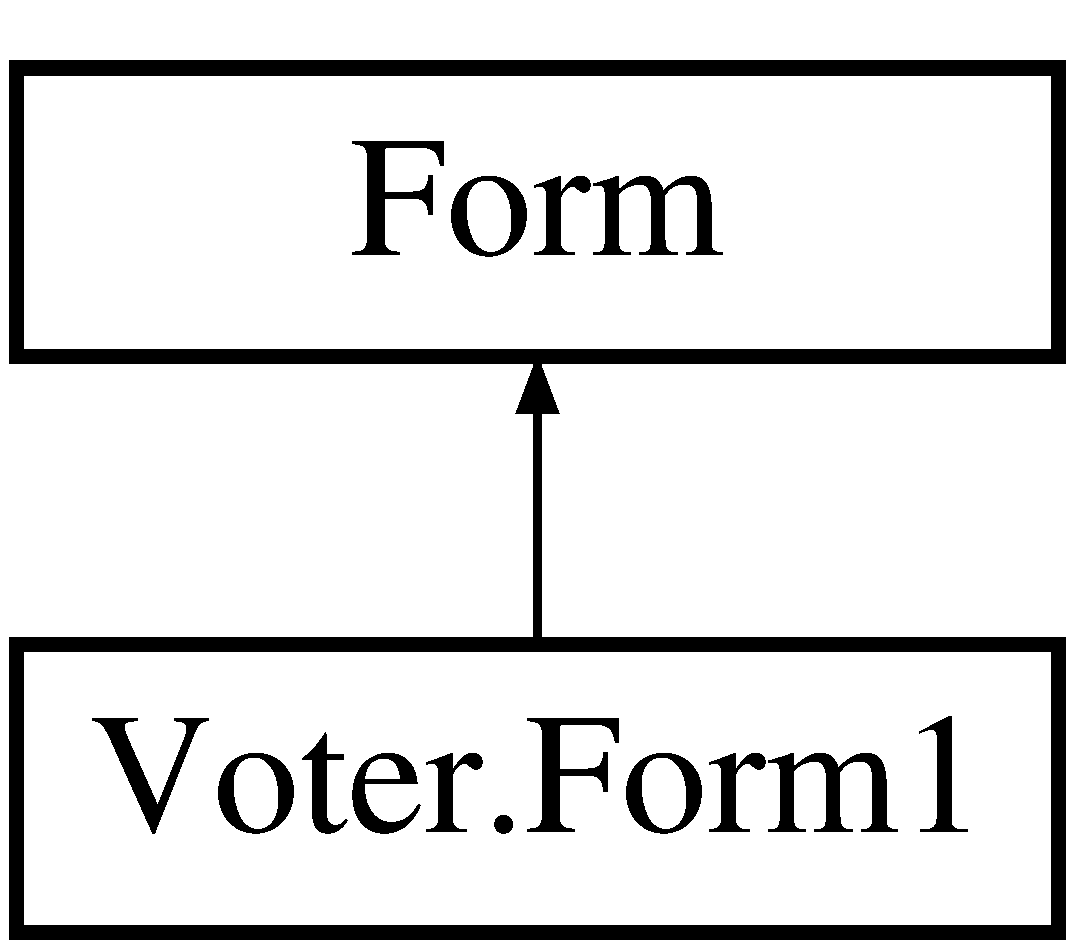
\includegraphics[height=2.000000cm]{class_voter_1_1_form1}
\end{center}
\end{figure}
\subsection*{Public Member Functions}
\begin{DoxyCompactItemize}
\item 
\hyperlink{class_voter_1_1_form1_a9d2419fe5a38bf455e7748b97c8b822c}{Form1} ()
\begin{DoxyCompactList}\small\item\em constructor of form \end{DoxyCompactList}\item 
void \hyperlink{class_voter_1_1_form1_a57dbc9331963aca6a28c141e2ce10276}{disable\+S\+L\+And\+S\+R\+Button} ()
\begin{DoxyCompactList}\small\item\em disable S\+L and S\+R buttons \end{DoxyCompactList}\item 
void \hyperlink{class_voter_1_1_form1_a9894005297c9c2837e59173c4fe57ad7}{disable\+Conection\+Proxy\+Button} ()
\begin{DoxyCompactList}\small\item\em disable connection with Proxy button \end{DoxyCompactList}\item 
void \hyperlink{class_voter_1_1_form1_a52871090531374025dbf70591855706f}{disable\+Connection\+E\+A\+Button} ()
\begin{DoxyCompactList}\small\item\em disable connection with Election Authority button \end{DoxyCompactList}\item 
void \hyperlink{class_voter_1_1_form1_aa1aea95e72637894339d9dfb6d386ef6}{disable\+Get\+Candidate\+List\+Button} ()
\begin{DoxyCompactList}\small\item\em disable Get Candidate List button \end{DoxyCompactList}\end{DoxyCompactItemize}
\subsection*{Protected Member Functions}
\begin{DoxyCompactItemize}
\item 
override void \hyperlink{class_voter_1_1_form1_abbf758d7a18bf7b34f41a46f021d747e}{Dispose} (bool disposing)
\begin{DoxyCompactList}\small\item\em Clean up any resources being used. \end{DoxyCompactList}\end{DoxyCompactItemize}
\subsection*{Properties}
\begin{DoxyCompactItemize}
\item 
List$<$ Text\+Box $>$ \hyperlink{class_voter_1_1_form1_a5c5e90b6fa99ecbaec0ee5b7d48f4d1d}{Text\+Boxes}\hspace{0.3cm}{\ttfamily  \mbox{[}get\mbox{]}}
\begin{DoxyCompactList}\small\item\em Text\+Boxes property which allow to get the list \end{DoxyCompactList}\item 
List$<$ Button\mbox{[}$\,$\mbox{]}$>$ \hyperlink{class_voter_1_1_form1_aa1ad45e2e705942b18168e5bb6a96d53}{Vote\+Buttons}\hspace{0.3cm}{\ttfamily  \mbox{[}get\mbox{]}}
\begin{DoxyCompactList}\small\item\em Vote\+Buttons property which allow to get the list \end{DoxyCompactList}\item 
int \hyperlink{class_voter_1_1_form1_a1a9fce02a2bbdbf9d3008b02b3b79bae}{conf\+Box}\hspace{0.3cm}{\ttfamily  \mbox{[}get, set\mbox{]}}
\begin{DoxyCompactList}\small\item\em conf\+Box property which allow to set and get value of confirmation box \end{DoxyCompactList}\end{DoxyCompactItemize}


\subsection{Detailed Description}
graphical user interface 



\subsection{Constructor \& Destructor Documentation}
\hypertarget{class_voter_1_1_form1_a9d2419fe5a38bf455e7748b97c8b822c}{}\index{Voter\+::\+Form1@{Voter\+::\+Form1}!Form1@{Form1}}
\index{Form1@{Form1}!Voter\+::\+Form1@{Voter\+::\+Form1}}
\subsubsection[{Form1}]{\setlength{\rightskip}{0pt plus 5cm}Voter.\+Form1.\+Form1 (
\begin{DoxyParamCaption}
{}
\end{DoxyParamCaption}
)\hspace{0.3cm}{\ttfamily [inline]}}\label{class_voter_1_1_form1_a9d2419fe5a38bf455e7748b97c8b822c}


constructor of form 



\subsection{Member Function Documentation}
\hypertarget{class_voter_1_1_form1_a9894005297c9c2837e59173c4fe57ad7}{}\index{Voter\+::\+Form1@{Voter\+::\+Form1}!disable\+Conection\+Proxy\+Button@{disable\+Conection\+Proxy\+Button}}
\index{disable\+Conection\+Proxy\+Button@{disable\+Conection\+Proxy\+Button}!Voter\+::\+Form1@{Voter\+::\+Form1}}
\subsubsection[{disable\+Conection\+Proxy\+Button}]{\setlength{\rightskip}{0pt plus 5cm}void Voter.\+Form1.\+disable\+Conection\+Proxy\+Button (
\begin{DoxyParamCaption}
{}
\end{DoxyParamCaption}
)\hspace{0.3cm}{\ttfamily [inline]}}\label{class_voter_1_1_form1_a9894005297c9c2837e59173c4fe57ad7}


disable connection with Proxy button 

\hypertarget{class_voter_1_1_form1_a52871090531374025dbf70591855706f}{}\index{Voter\+::\+Form1@{Voter\+::\+Form1}!disable\+Connection\+E\+A\+Button@{disable\+Connection\+E\+A\+Button}}
\index{disable\+Connection\+E\+A\+Button@{disable\+Connection\+E\+A\+Button}!Voter\+::\+Form1@{Voter\+::\+Form1}}
\subsubsection[{disable\+Connection\+E\+A\+Button}]{\setlength{\rightskip}{0pt plus 5cm}void Voter.\+Form1.\+disable\+Connection\+E\+A\+Button (
\begin{DoxyParamCaption}
{}
\end{DoxyParamCaption}
)\hspace{0.3cm}{\ttfamily [inline]}}\label{class_voter_1_1_form1_a52871090531374025dbf70591855706f}


disable connection with Election Authority button 

\hypertarget{class_voter_1_1_form1_aa1aea95e72637894339d9dfb6d386ef6}{}\index{Voter\+::\+Form1@{Voter\+::\+Form1}!disable\+Get\+Candidate\+List\+Button@{disable\+Get\+Candidate\+List\+Button}}
\index{disable\+Get\+Candidate\+List\+Button@{disable\+Get\+Candidate\+List\+Button}!Voter\+::\+Form1@{Voter\+::\+Form1}}
\subsubsection[{disable\+Get\+Candidate\+List\+Button}]{\setlength{\rightskip}{0pt plus 5cm}void Voter.\+Form1.\+disable\+Get\+Candidate\+List\+Button (
\begin{DoxyParamCaption}
{}
\end{DoxyParamCaption}
)\hspace{0.3cm}{\ttfamily [inline]}}\label{class_voter_1_1_form1_aa1aea95e72637894339d9dfb6d386ef6}


disable Get Candidate List button 

\hypertarget{class_voter_1_1_form1_a57dbc9331963aca6a28c141e2ce10276}{}\index{Voter\+::\+Form1@{Voter\+::\+Form1}!disable\+S\+L\+And\+S\+R\+Button@{disable\+S\+L\+And\+S\+R\+Button}}
\index{disable\+S\+L\+And\+S\+R\+Button@{disable\+S\+L\+And\+S\+R\+Button}!Voter\+::\+Form1@{Voter\+::\+Form1}}
\subsubsection[{disable\+S\+L\+And\+S\+R\+Button}]{\setlength{\rightskip}{0pt plus 5cm}void Voter.\+Form1.\+disable\+S\+L\+And\+S\+R\+Button (
\begin{DoxyParamCaption}
{}
\end{DoxyParamCaption}
)\hspace{0.3cm}{\ttfamily [inline]}}\label{class_voter_1_1_form1_a57dbc9331963aca6a28c141e2ce10276}


disable S\+L and S\+R buttons 

\hypertarget{class_voter_1_1_form1_abbf758d7a18bf7b34f41a46f021d747e}{}\index{Voter\+::\+Form1@{Voter\+::\+Form1}!Dispose@{Dispose}}
\index{Dispose@{Dispose}!Voter\+::\+Form1@{Voter\+::\+Form1}}
\subsubsection[{Dispose}]{\setlength{\rightskip}{0pt plus 5cm}override void Voter.\+Form1.\+Dispose (
\begin{DoxyParamCaption}
\item[{bool}]{disposing}
\end{DoxyParamCaption}
)\hspace{0.3cm}{\ttfamily [inline]}, {\ttfamily [protected]}}\label{class_voter_1_1_form1_abbf758d7a18bf7b34f41a46f021d747e}


Clean up any resources being used. 


\begin{DoxyParams}{Parameters}
{\em disposing} & true if managed resources should be disposed; otherwise, false.\\
\hline
\end{DoxyParams}


\subsection{Property Documentation}
\hypertarget{class_voter_1_1_form1_a1a9fce02a2bbdbf9d3008b02b3b79bae}{}\index{Voter\+::\+Form1@{Voter\+::\+Form1}!conf\+Box@{conf\+Box}}
\index{conf\+Box@{conf\+Box}!Voter\+::\+Form1@{Voter\+::\+Form1}}
\subsubsection[{conf\+Box}]{\setlength{\rightskip}{0pt plus 5cm}int Voter.\+Form1.\+conf\+Box\hspace{0.3cm}{\ttfamily [get]}, {\ttfamily [set]}}\label{class_voter_1_1_form1_a1a9fce02a2bbdbf9d3008b02b3b79bae}


conf\+Box property which allow to set and get value of confirmation box 

\hypertarget{class_voter_1_1_form1_a5c5e90b6fa99ecbaec0ee5b7d48f4d1d}{}\index{Voter\+::\+Form1@{Voter\+::\+Form1}!Text\+Boxes@{Text\+Boxes}}
\index{Text\+Boxes@{Text\+Boxes}!Voter\+::\+Form1@{Voter\+::\+Form1}}
\subsubsection[{Text\+Boxes}]{\setlength{\rightskip}{0pt plus 5cm}List$<$Text\+Box$>$ Voter.\+Form1.\+Text\+Boxes\hspace{0.3cm}{\ttfamily [get]}}\label{class_voter_1_1_form1_a5c5e90b6fa99ecbaec0ee5b7d48f4d1d}


Text\+Boxes property which allow to get the list 

\hypertarget{class_voter_1_1_form1_aa1ad45e2e705942b18168e5bb6a96d53}{}\index{Voter\+::\+Form1@{Voter\+::\+Form1}!Vote\+Buttons@{Vote\+Buttons}}
\index{Vote\+Buttons@{Vote\+Buttons}!Voter\+::\+Form1@{Voter\+::\+Form1}}
\subsubsection[{Vote\+Buttons}]{\setlength{\rightskip}{0pt plus 5cm}List$<$Button\mbox{[}$\,$\mbox{]}$>$ Voter.\+Form1.\+Vote\+Buttons\hspace{0.3cm}{\ttfamily [get]}}\label{class_voter_1_1_form1_aa1ad45e2e705942b18168e5bb6a96d53}


Vote\+Buttons property which allow to get the list 



The documentation for this class was generated from the following files\+:\begin{DoxyCompactItemize}
\item 
Voter/\+Voter/Form1.\+cs\item 
Voter/\+Voter/Form1.\+Designer.\+cs\end{DoxyCompactItemize}

\hypertarget{class_voter_1_1_logs}{}\section{Voter.\+Logs Class Reference}
\label{class_voter_1_1_logs}\index{Voter.\+Logs@{Voter.\+Logs}}


allows to collect and display logs  


\subsection*{Public Member Functions}
\begin{DoxyCompactItemize}
\item 
\hyperlink{class_voter_1_1_logs_a37904e9fa4c48bcc1a540c6685484e7d}{Logs} (List\+View logs\+List\+View)
\begin{DoxyCompactList}\small\item\em \hyperlink{class_voter_1_1_logs}{Logs} instance\textquotesingle{}s constructor \end{DoxyCompactList}\item 
void \hyperlink{class_voter_1_1_logs_aac5ba38a4fecfd5026d039969e05a2ed}{add\+Log} (string log, bool time, int flag, bool another\+Thread=false)
\begin{DoxyCompactList}\small\item\em adds log \end{DoxyCompactList}\end{DoxyCompactItemize}
\subsection*{Properties}
\begin{DoxyCompactItemize}
\item 
\hypertarget{class_voter_1_1_logs_a9252e7d84515eb59a4b0ff9c4cc09156}{}string {\bfseries Voter\+Name}\hspace{0.3cm}{\ttfamily  \mbox{[}get, set\mbox{]}}\label{class_voter_1_1_logs_a9252e7d84515eb59a4b0ff9c4cc09156}

\end{DoxyCompactItemize}


\subsection{Detailed Description}
allows to collect and display logs 



\subsection{Constructor \& Destructor Documentation}
\hypertarget{class_voter_1_1_logs_a37904e9fa4c48bcc1a540c6685484e7d}{}\index{Voter\+::\+Logs@{Voter\+::\+Logs}!Logs@{Logs}}
\index{Logs@{Logs}!Voter\+::\+Logs@{Voter\+::\+Logs}}
\subsubsection[{Logs}]{\setlength{\rightskip}{0pt plus 5cm}Voter.\+Logs.\+Logs (
\begin{DoxyParamCaption}
\item[{List\+View}]{logs\+List\+View}
\end{DoxyParamCaption}
)\hspace{0.3cm}{\ttfamily [inline]}}\label{class_voter_1_1_logs_a37904e9fa4c48bcc1a540c6685484e7d}


\hyperlink{class_voter_1_1_logs}{Logs} instance\textquotesingle{}s constructor 


\begin{DoxyParams}{Parameters}
{\em logs\+List\+View} & logs list view\\
\hline
\end{DoxyParams}


\subsection{Member Function Documentation}
\hypertarget{class_voter_1_1_logs_aac5ba38a4fecfd5026d039969e05a2ed}{}\index{Voter\+::\+Logs@{Voter\+::\+Logs}!add\+Log@{add\+Log}}
\index{add\+Log@{add\+Log}!Voter\+::\+Logs@{Voter\+::\+Logs}}
\subsubsection[{add\+Log}]{\setlength{\rightskip}{0pt plus 5cm}void Voter.\+Logs.\+add\+Log (
\begin{DoxyParamCaption}
\item[{string}]{log, }
\item[{bool}]{time, }
\item[{int}]{flag, }
\item[{bool}]{another\+Thread = {\ttfamily false}}
\end{DoxyParamCaption}
)\hspace{0.3cm}{\ttfamily [inline]}}\label{class_voter_1_1_logs_aac5ba38a4fecfd5026d039969e05a2ed}


adds log 


\begin{DoxyParams}{Parameters}
{\em log} & log message\\
\hline
{\em time} & if print time\\
\hline
{\em flag} & type of message (error, info...)\\
\hline
{\em another\+Thread} & thread flag\\
\hline
\end{DoxyParams}


The documentation for this class was generated from the following file\+:\begin{DoxyCompactItemize}
\item 
Voter/\+Voter/Logs.\+cs\end{DoxyCompactItemize}

\hypertarget{class_voter_1_1_parser}{}\section{Voter.\+Parser Class Reference}
\label{class_voter_1_1_parser}\index{Voter.\+Parser@{Voter.\+Parser}}


parsing recived messages  


\subsection*{Public Member Functions}
\begin{DoxyCompactItemize}
\item 
\hyperlink{class_voter_1_1_parser_a5982183425367d54cbb59d41d26ff350}{Parser} (\hyperlink{class_voter_1_1_logs}{Logs} logs, \hyperlink{class_voter_1_1_voter}{Voter} voter)
\begin{DoxyCompactList}\small\item\em parser\textquotesingle{}s constructor \end{DoxyCompactList}\item 
void \hyperlink{class_voter_1_1_parser_a228efa172bfe6e9e0a763750a5dfe6cb}{parse\+Message} (string msg)
\begin{DoxyCompactList}\small\item\em parses message \end{DoxyCompactList}\end{DoxyCompactItemize}


\subsection{Detailed Description}
parsing recived messages 



\subsection{Constructor \& Destructor Documentation}
\hypertarget{class_voter_1_1_parser_a5982183425367d54cbb59d41d26ff350}{}\index{Voter\+::\+Parser@{Voter\+::\+Parser}!Parser@{Parser}}
\index{Parser@{Parser}!Voter\+::\+Parser@{Voter\+::\+Parser}}
\subsubsection[{Parser}]{\setlength{\rightskip}{0pt plus 5cm}Voter.\+Parser.\+Parser (
\begin{DoxyParamCaption}
\item[{{\bf Logs}}]{logs, }
\item[{{\bf Voter}}]{voter}
\end{DoxyParamCaption}
)\hspace{0.3cm}{\ttfamily [inline]}}\label{class_voter_1_1_parser_a5982183425367d54cbb59d41d26ff350}


parser\textquotesingle{}s constructor 


\begin{DoxyParams}{Parameters}
{\em logs} & log instance\\
\hline
{\em voter} & voter instance\\
\hline
\end{DoxyParams}


\subsection{Member Function Documentation}
\hypertarget{class_voter_1_1_parser_a228efa172bfe6e9e0a763750a5dfe6cb}{}\index{Voter\+::\+Parser@{Voter\+::\+Parser}!parse\+Message@{parse\+Message}}
\index{parse\+Message@{parse\+Message}!Voter\+::\+Parser@{Voter\+::\+Parser}}
\subsubsection[{parse\+Message}]{\setlength{\rightskip}{0pt plus 5cm}void Voter.\+Parser.\+parse\+Message (
\begin{DoxyParamCaption}
\item[{string}]{msg}
\end{DoxyParamCaption}
)\hspace{0.3cm}{\ttfamily [inline]}}\label{class_voter_1_1_parser_a228efa172bfe6e9e0a763750a5dfe6cb}


parses message 


\begin{DoxyParams}{Parameters}
{\em msg} & recived message\\
\hline
\end{DoxyParams}
\begin{DoxyReturn}{Returns}
parsing result
\end{DoxyReturn}


The documentation for this class was generated from the following file\+:\begin{DoxyCompactItemize}
\item 
Voter/\+Voter/Parser.\+cs\end{DoxyCompactItemize}

\hypertarget{class_voter_1_1_voter}{}\section{Voter.\+Voter Class Reference}
\label{class_voter_1_1_voter}\index{Voter.\+Voter@{Voter.\+Voter}}


\hyperlink{class_voter_1_1_voter}{Voter} class -\/ getting vote from person  


\subsection*{Public Member Functions}
\begin{DoxyCompactItemize}
\item 
\hyperlink{class_voter_1_1_voter_a659d64924100badf22d6e4ab6b27b10b}{Voter} (\hyperlink{class_voter_1_1_logs}{Logs} logs, \hyperlink{class_voter_1_1_configuration}{Configuration} configuration, \hyperlink{class_voter_1_1_form1}{Form1} form, \hyperlink{class_voter_1_1_confirmation}{Confirmation} confirm)
\begin{DoxyCompactList}\small\item\em constructor \end{DoxyCompactList}\item 
void \hyperlink{class_voter_1_1_voter_a4c06e89ca81067c0f8e405bc3bbc1946}{request\+For\+S\+Land\+S\+R} ()
\begin{DoxyCompactList}\small\item\em request for S\+L and S\+R (voter to proxy) \end{DoxyCompactList}\item 
void \hyperlink{class_voter_1_1_voter_ad45bb52a29505df92a2a8d877cb75c03}{disable\+S\+L\+And\+S\+R\+Button} ()
\begin{DoxyCompactList}\small\item\em disable S\+L and S\+R getting button \end{DoxyCompactList}\item 
void \hyperlink{class_voter_1_1_voter_a15b6ebde39984a8447164bffdabf2718}{request\+For\+Candidates\+List} ()
\begin{DoxyCompactList}\small\item\em request for candidate list (voter to E\+A) \end{DoxyCompactList}\item 
void \hyperlink{class_voter_1_1_voter_a75978572b738eddd7af0e74823683585}{disable\+Connection\+Proxy\+Button} ()
\begin{DoxyCompactList}\small\item\em disable connection to proxy button \end{DoxyCompactList}\item 
void \hyperlink{class_voter_1_1_voter_a3e4b06943a2792a4c39de67e431ed6af}{disable\+Connection\+E\+A\+Button} ()
\begin{DoxyCompactList}\small\item\em disable connection to ea button \end{DoxyCompactList}\item 
void \hyperlink{class_voter_1_1_voter_a254426e5a240b96c33a8291b1ea75a87}{save\+Candidate\+List} (string msg)
\begin{DoxyCompactList}\small\item\em saves cadidates list \end{DoxyCompactList}\item 
void \hyperlink{class_voter_1_1_voter_a127f8b0f9a0e29e2153f95f669ed60bb}{send\+Vote\+To\+Proxy} ()
\begin{DoxyCompactList}\small\item\em sends vote to proxy (ie. message\+: V\+O\+T\+E\& Voter\+\_\+name;1\+:0\+:0\+:0;1\+:0\+:0\+:0;0\+:0\+:0\+:1;0\+:0\+:0\+:1;0\+:0\+:0\+:1) \end{DoxyCompactList}\item 
void \hyperlink{class_voter_1_1_voter_afd102d94d3bb4bc3e3b5369e0de299f8}{set\+Confirm} (int column)
\begin{DoxyCompactList}\small\item\em sets confirmation \end{DoxyCompactList}\item 
void \hyperlink{class_voter_1_1_voter_a533531950023f29d27d8f676f6a290bb}{save\+Signed\+Column\+And\+Token} (string message)
\begin{DoxyCompactList}\small\item\em save signed column and token \end{DoxyCompactList}\end{DoxyCompactItemize}
\subsection*{Properties}
\begin{DoxyCompactItemize}
\item 
\hypertarget{class_voter_1_1_voter_a7472e51003adaa6d920ff9554ef53067}{}\hyperlink{class_voter_1_1_client}{Client} {\bfseries Proxy\+Client}\hspace{0.3cm}{\ttfamily  \mbox{[}get\mbox{]}}\label{class_voter_1_1_voter_a7472e51003adaa6d920ff9554ef53067}

\item 
\hypertarget{class_voter_1_1_voter_a4487e93cfddf755f140b53f5c03c920b}{}\hyperlink{class_voter_1_1_client}{Client} {\bfseries Election\+Authority\+Client}\hspace{0.3cm}{\ttfamily  \mbox{[}get\mbox{]}}\label{class_voter_1_1_voter_a4487e93cfddf755f140b53f5c03c920b}

\item 
\hypertarget{class_voter_1_1_voter_ad36bc1966b65f0b94cf135d172b93c02}{}\hyperlink{class_voter_1_1_voter_ballot}{Voter\+Ballot} {\bfseries Voter\+Ballot}\hspace{0.3cm}{\ttfamily  \mbox{[}get\mbox{]}}\label{class_voter_1_1_voter_ad36bc1966b65f0b94cf135d172b93c02}

\end{DoxyCompactItemize}


\subsection{Detailed Description}
\hyperlink{class_voter_1_1_voter}{Voter} class -\/ getting vote from person 



\subsection{Constructor \& Destructor Documentation}
\hypertarget{class_voter_1_1_voter_a659d64924100badf22d6e4ab6b27b10b}{}\index{Voter\+::\+Voter@{Voter\+::\+Voter}!Voter@{Voter}}
\index{Voter@{Voter}!Voter\+::\+Voter@{Voter\+::\+Voter}}
\subsubsection[{Voter}]{\setlength{\rightskip}{0pt plus 5cm}Voter.\+Voter.\+Voter (
\begin{DoxyParamCaption}
\item[{{\bf Logs}}]{logs, }
\item[{{\bf Configuration}}]{configuration, }
\item[{{\bf Form1}}]{form, }
\item[{{\bf Confirmation}}]{confirm}
\end{DoxyParamCaption}
)\hspace{0.3cm}{\ttfamily [inline]}}\label{class_voter_1_1_voter_a659d64924100badf22d6e4ab6b27b10b}


constructor 


\begin{DoxyParams}{Parameters}
{\em logs} & log instance\\
\hline
{\em configuration} & configuration loaded\\
\hline
{\em form} & form application\\
\hline
{\em confirm} & confirmation for voter\\
\hline
\end{DoxyParams}


\subsection{Member Function Documentation}
\hypertarget{class_voter_1_1_voter_a3e4b06943a2792a4c39de67e431ed6af}{}\index{Voter\+::\+Voter@{Voter\+::\+Voter}!disable\+Connection\+E\+A\+Button@{disable\+Connection\+E\+A\+Button}}
\index{disable\+Connection\+E\+A\+Button@{disable\+Connection\+E\+A\+Button}!Voter\+::\+Voter@{Voter\+::\+Voter}}
\subsubsection[{disable\+Connection\+E\+A\+Button}]{\setlength{\rightskip}{0pt plus 5cm}void Voter.\+Voter.\+disable\+Connection\+E\+A\+Button (
\begin{DoxyParamCaption}
{}
\end{DoxyParamCaption}
)\hspace{0.3cm}{\ttfamily [inline]}}\label{class_voter_1_1_voter_a3e4b06943a2792a4c39de67e431ed6af}


disable connection to ea button 

\hypertarget{class_voter_1_1_voter_a75978572b738eddd7af0e74823683585}{}\index{Voter\+::\+Voter@{Voter\+::\+Voter}!disable\+Connection\+Proxy\+Button@{disable\+Connection\+Proxy\+Button}}
\index{disable\+Connection\+Proxy\+Button@{disable\+Connection\+Proxy\+Button}!Voter\+::\+Voter@{Voter\+::\+Voter}}
\subsubsection[{disable\+Connection\+Proxy\+Button}]{\setlength{\rightskip}{0pt plus 5cm}void Voter.\+Voter.\+disable\+Connection\+Proxy\+Button (
\begin{DoxyParamCaption}
{}
\end{DoxyParamCaption}
)\hspace{0.3cm}{\ttfamily [inline]}}\label{class_voter_1_1_voter_a75978572b738eddd7af0e74823683585}


disable connection to proxy button 

\hypertarget{class_voter_1_1_voter_ad45bb52a29505df92a2a8d877cb75c03}{}\index{Voter\+::\+Voter@{Voter\+::\+Voter}!disable\+S\+L\+And\+S\+R\+Button@{disable\+S\+L\+And\+S\+R\+Button}}
\index{disable\+S\+L\+And\+S\+R\+Button@{disable\+S\+L\+And\+S\+R\+Button}!Voter\+::\+Voter@{Voter\+::\+Voter}}
\subsubsection[{disable\+S\+L\+And\+S\+R\+Button}]{\setlength{\rightskip}{0pt plus 5cm}void Voter.\+Voter.\+disable\+S\+L\+And\+S\+R\+Button (
\begin{DoxyParamCaption}
{}
\end{DoxyParamCaption}
)\hspace{0.3cm}{\ttfamily [inline]}}\label{class_voter_1_1_voter_ad45bb52a29505df92a2a8d877cb75c03}


disable S\+L and S\+R getting button 

\hypertarget{class_voter_1_1_voter_a15b6ebde39984a8447164bffdabf2718}{}\index{Voter\+::\+Voter@{Voter\+::\+Voter}!request\+For\+Candidates\+List@{request\+For\+Candidates\+List}}
\index{request\+For\+Candidates\+List@{request\+For\+Candidates\+List}!Voter\+::\+Voter@{Voter\+::\+Voter}}
\subsubsection[{request\+For\+Candidates\+List}]{\setlength{\rightskip}{0pt plus 5cm}void Voter.\+Voter.\+request\+For\+Candidates\+List (
\begin{DoxyParamCaption}
{}
\end{DoxyParamCaption}
)\hspace{0.3cm}{\ttfamily [inline]}}\label{class_voter_1_1_voter_a15b6ebde39984a8447164bffdabf2718}


request for candidate list (voter to E\+A) 

\hypertarget{class_voter_1_1_voter_a4c06e89ca81067c0f8e405bc3bbc1946}{}\index{Voter\+::\+Voter@{Voter\+::\+Voter}!request\+For\+S\+Land\+S\+R@{request\+For\+S\+Land\+S\+R}}
\index{request\+For\+S\+Land\+S\+R@{request\+For\+S\+Land\+S\+R}!Voter\+::\+Voter@{Voter\+::\+Voter}}
\subsubsection[{request\+For\+S\+Land\+S\+R}]{\setlength{\rightskip}{0pt plus 5cm}void Voter.\+Voter.\+request\+For\+S\+Land\+S\+R (
\begin{DoxyParamCaption}
{}
\end{DoxyParamCaption}
)\hspace{0.3cm}{\ttfamily [inline]}}\label{class_voter_1_1_voter_a4c06e89ca81067c0f8e405bc3bbc1946}


request for S\+L and S\+R (voter to proxy) 

\hypertarget{class_voter_1_1_voter_a254426e5a240b96c33a8291b1ea75a87}{}\index{Voter\+::\+Voter@{Voter\+::\+Voter}!save\+Candidate\+List@{save\+Candidate\+List}}
\index{save\+Candidate\+List@{save\+Candidate\+List}!Voter\+::\+Voter@{Voter\+::\+Voter}}
\subsubsection[{save\+Candidate\+List}]{\setlength{\rightskip}{0pt plus 5cm}void Voter.\+Voter.\+save\+Candidate\+List (
\begin{DoxyParamCaption}
\item[{string}]{msg}
\end{DoxyParamCaption}
)\hspace{0.3cm}{\ttfamily [inline]}}\label{class_voter_1_1_voter_a254426e5a240b96c33a8291b1ea75a87}


saves cadidates list 


\begin{DoxyParams}{Parameters}
{\em msg} & recived message\\
\hline
\end{DoxyParams}
\hypertarget{class_voter_1_1_voter_a533531950023f29d27d8f676f6a290bb}{}\index{Voter\+::\+Voter@{Voter\+::\+Voter}!save\+Signed\+Column\+And\+Token@{save\+Signed\+Column\+And\+Token}}
\index{save\+Signed\+Column\+And\+Token@{save\+Signed\+Column\+And\+Token}!Voter\+::\+Voter@{Voter\+::\+Voter}}
\subsubsection[{save\+Signed\+Column\+And\+Token}]{\setlength{\rightskip}{0pt plus 5cm}void Voter.\+Voter.\+save\+Signed\+Column\+And\+Token (
\begin{DoxyParamCaption}
\item[{string}]{message}
\end{DoxyParamCaption}
)\hspace{0.3cm}{\ttfamily [inline]}}\label{class_voter_1_1_voter_a533531950023f29d27d8f676f6a290bb}


save signed column and token 


\begin{DoxyParams}{Parameters}
{\em message} & recived message\\
\hline
\end{DoxyParams}
\hypertarget{class_voter_1_1_voter_a127f8b0f9a0e29e2153f95f669ed60bb}{}\index{Voter\+::\+Voter@{Voter\+::\+Voter}!send\+Vote\+To\+Proxy@{send\+Vote\+To\+Proxy}}
\index{send\+Vote\+To\+Proxy@{send\+Vote\+To\+Proxy}!Voter\+::\+Voter@{Voter\+::\+Voter}}
\subsubsection[{send\+Vote\+To\+Proxy}]{\setlength{\rightskip}{0pt plus 5cm}void Voter.\+Voter.\+send\+Vote\+To\+Proxy (
\begin{DoxyParamCaption}
{}
\end{DoxyParamCaption}
)\hspace{0.3cm}{\ttfamily [inline]}}\label{class_voter_1_1_voter_a127f8b0f9a0e29e2153f95f669ed60bb}


sends vote to proxy (ie. message\+: V\+O\+T\+E\& Voter\+\_\+name;1\+:0\+:0\+:0;1\+:0\+:0\+:0;0\+:0\+:0\+:1;0\+:0\+:0\+:1;0\+:0\+:0\+:1) 

\hypertarget{class_voter_1_1_voter_afd102d94d3bb4bc3e3b5369e0de299f8}{}\index{Voter\+::\+Voter@{Voter\+::\+Voter}!set\+Confirm@{set\+Confirm}}
\index{set\+Confirm@{set\+Confirm}!Voter\+::\+Voter@{Voter\+::\+Voter}}
\subsubsection[{set\+Confirm}]{\setlength{\rightskip}{0pt plus 5cm}void Voter.\+Voter.\+set\+Confirm (
\begin{DoxyParamCaption}
\item[{int}]{column}
\end{DoxyParamCaption}
)\hspace{0.3cm}{\ttfamily [inline]}}\label{class_voter_1_1_voter_afd102d94d3bb4bc3e3b5369e0de299f8}


sets confirmation 


\begin{DoxyParams}{Parameters}
{\em column} & confirmation column choosed by voter\\
\hline
\end{DoxyParams}


The documentation for this class was generated from the following file\+:\begin{DoxyCompactItemize}
\item 
Voter/\+Voter/Voter.\+cs\end{DoxyCompactItemize}

\hypertarget{class_voter_1_1_voter_ballot}{}\section{Voter.\+Voter\+Ballot Class Reference}
\label{class_voter_1_1_voter_ballot}\index{Voter.\+Voter\+Ballot@{Voter.\+Voter\+Ballot}}


\hyperlink{class_voter_1_1_voter}{Voter} ballot (vote\textquotesingle{}s data as S\+L, S\+R, vote, yes/no position)  


\subsection*{Public Member Functions}
\begin{DoxyCompactItemize}
\item 
\hyperlink{class_voter_1_1_voter_ballot_a78ca278f7add21b16e29b4f91569812e}{Voter\+Ballot} (int numb\+Of\+Cand)
\begin{DoxyCompactList}\small\item\em constructor \end{DoxyCompactList}\item 
bool \hyperlink{class_voter_1_1_voter_ballot_af73eb9545b6259715cea0a22f6a1c80f}{vote} (int x, int y)
\begin{DoxyCompactList}\small\item\em try-\/to-\/vote for x,y position \end{DoxyCompactList}\item 
bool \hyperlink{class_voter_1_1_voter_ballot_a00763bb4933a65ec908aedad2634ee05}{vote\+Done} ()
\begin{DoxyCompactList}\small\item\em checks if voting is done \end{DoxyCompactList}\end{DoxyCompactItemize}
\subsection*{Properties}
\begin{DoxyCompactItemize}
\item 
\hypertarget{class_voter_1_1_voter_ballot_a8c7c5487fc638872fd9f9cbe9fd12bc3}{}int\mbox{[},\mbox{]} {\bfseries Voted}\hspace{0.3cm}{\ttfamily  \mbox{[}get\mbox{]}}\label{class_voter_1_1_voter_ballot_a8c7c5487fc638872fd9f9cbe9fd12bc3}

\item 
\hypertarget{class_voter_1_1_voter_ballot_aa591a90931ed53d539117425897b6528}{}Big\+Integer {\bfseries S\+L}\hspace{0.3cm}{\ttfamily  \mbox{[}get, set\mbox{]}}\label{class_voter_1_1_voter_ballot_aa591a90931ed53d539117425897b6528}

\item 
\hypertarget{class_voter_1_1_voter_ballot_a1b4aec46e919986eae6202c860f9c6e5}{}Big\+Integer {\bfseries S\+R}\hspace{0.3cm}{\ttfamily  \mbox{[}get, set\mbox{]}}\label{class_voter_1_1_voter_ballot_a1b4aec46e919986eae6202c860f9c6e5}

\item 
\hypertarget{class_voter_1_1_voter_ballot_a537baffdb84d11dbd93aa356f3382b27}{}Big\+Integer {\bfseries Token}\hspace{0.3cm}{\ttfamily  \mbox{[}get, set\mbox{]}}\label{class_voter_1_1_voter_ballot_a537baffdb84d11dbd93aa356f3382b27}

\item 
\hypertarget{class_voter_1_1_voter_ballot_a32511f4dcc46ee028f82d0bdb28eb6ba}{}Big\+Integer {\bfseries Signed\+Blind\+Column}\hspace{0.3cm}{\ttfamily  \mbox{[}get, set\mbox{]}}\label{class_voter_1_1_voter_ballot_a32511f4dcc46ee028f82d0bdb28eb6ba}

\end{DoxyCompactItemize}


\subsection{Detailed Description}
\hyperlink{class_voter_1_1_voter}{Voter} ballot (vote\textquotesingle{}s data as S\+L, S\+R, vote, yes/no position) 



\subsection{Constructor \& Destructor Documentation}
\hypertarget{class_voter_1_1_voter_ballot_a78ca278f7add21b16e29b4f91569812e}{}\index{Voter\+::\+Voter\+Ballot@{Voter\+::\+Voter\+Ballot}!Voter\+Ballot@{Voter\+Ballot}}
\index{Voter\+Ballot@{Voter\+Ballot}!Voter\+::\+Voter\+Ballot@{Voter\+::\+Voter\+Ballot}}
\subsubsection[{Voter\+Ballot}]{\setlength{\rightskip}{0pt plus 5cm}Voter.\+Voter\+Ballot.\+Voter\+Ballot (
\begin{DoxyParamCaption}
\item[{int}]{numb\+Of\+Cand}
\end{DoxyParamCaption}
)\hspace{0.3cm}{\ttfamily [inline]}}\label{class_voter_1_1_voter_ballot_a78ca278f7add21b16e29b4f91569812e}


constructor 


\begin{DoxyParams}{Parameters}
{\em numb\+Of\+Cand} & \\
\hline
\end{DoxyParams}


\subsection{Member Function Documentation}
\hypertarget{class_voter_1_1_voter_ballot_af73eb9545b6259715cea0a22f6a1c80f}{}\index{Voter\+::\+Voter\+Ballot@{Voter\+::\+Voter\+Ballot}!vote@{vote}}
\index{vote@{vote}!Voter\+::\+Voter\+Ballot@{Voter\+::\+Voter\+Ballot}}
\subsubsection[{vote}]{\setlength{\rightskip}{0pt plus 5cm}bool Voter.\+Voter\+Ballot.\+vote (
\begin{DoxyParamCaption}
\item[{int}]{x, }
\item[{int}]{y}
\end{DoxyParamCaption}
)\hspace{0.3cm}{\ttfamily [inline]}}\label{class_voter_1_1_voter_ballot_af73eb9545b6259715cea0a22f6a1c80f}


try-\/to-\/vote for x,y position 


\begin{DoxyParams}{Parameters}
{\em x} & 1st dimension\\
\hline
{\em y} & 2nd dimension\\
\hline
\end{DoxyParams}
\begin{DoxyReturn}{Returns}
result of try-\/to-\/vote action
\end{DoxyReturn}
\hypertarget{class_voter_1_1_voter_ballot_a00763bb4933a65ec908aedad2634ee05}{}\index{Voter\+::\+Voter\+Ballot@{Voter\+::\+Voter\+Ballot}!vote\+Done@{vote\+Done}}
\index{vote\+Done@{vote\+Done}!Voter\+::\+Voter\+Ballot@{Voter\+::\+Voter\+Ballot}}
\subsubsection[{vote\+Done}]{\setlength{\rightskip}{0pt plus 5cm}bool Voter.\+Voter\+Ballot.\+vote\+Done (
\begin{DoxyParamCaption}
{}
\end{DoxyParamCaption}
)\hspace{0.3cm}{\ttfamily [inline]}}\label{class_voter_1_1_voter_ballot_a00763bb4933a65ec908aedad2634ee05}


checks if voting is done 

\begin{DoxyReturn}{Returns}
if voting is done
\end{DoxyReturn}


The documentation for this class was generated from the following file\+:\begin{DoxyCompactItemize}
\item 
Voter/\+Voter/Voter\+Ballot.\+cs\end{DoxyCompactItemize}

%--- End generated contents ---

% Index
\backmatter
\newpage
\phantomsection
\clearemptydoublepage
\addcontentsline{toc}{chapter}{Index}
\printindex

\end{document}
